\chapter{Tidsrekkeanalyse og prediksjon}
\label{kap:tidsrekkeanalyse} % Opprinnelig kapittelnr: 13

\section{Innledning}

Mange statistiske undersøkelser har form av at samme størrelse
observeres på etterfølgende tidspunkter over en viss tid.  Slike
observasjoner kalles gjerne en {\em tidsrekke}.  Eksempler på tidsrekker
er 
\begin{itemize}
\item  Temperaturer målt på etterfølgende dager.
\item  Forurensing målt på etterfølgende dager.
\item  Omsetning i et varehus fra dag til dag.
\item  En prisindeks fra uke til uke.
\item  Sysselsetting fra måned til måned.
\item  Antall drepte i trafikken fra år til år.
\end{itemize}

En tidsrekke beskriver et utviklingsforløp, og formålet med en 
tidsrekkeanalyse kan være å forstå den utvikling som har funnet
sted.  Ofte vil det også være et underliggende ønske om å
bruke de funne resultater til å treffe beslutninger.  I forbindelse med
tidsrekkeanalyse kommer det derfor inn et moment av {\em prediksjon}, vi
ønsker å forutsi den videre utvikling av tidsrekken på grunnlag
av de observasjoner som er gjort opp til nå.

Ved analyse av tidsrekker kan man lete etter utviklingsmønstre og
typiske regulariteter.  De konklusjoner som eventuelt trekkes om fremtiden
av en slik analyse forutsetter at omstendighetene ikke
endrer seg drastisk i forhold til den tidsperioden vi har observasjoner fra.  
De beslutninger som treffes på grunnlag av en tidsrekkeanalyse kan ha
ulik natur.  Det kan være tale om å innrette seg etter en ventet
utvikling, eksempelvis når det gjelder å bestemme 
produksjonskvanta.  Det kan også være tale om å treffe tiltak for
å snu en uønsket utvikling som synes å inntreffe dersom en ikke
foretar seg noe, eksempelvis ved forurensingsproblemer.

En rekke ting er typiske for tidsrekker, vi vil spesielt trekke fram fire
elementer:

Vi kan ha en {\em trend} som gir uttrykk for langtidsutviklingen av 
tidsrekken.  I denne forbindelse taler vi gjerne om stigende eller fallende
trend.

\begin{figure}[ht]
\centering
   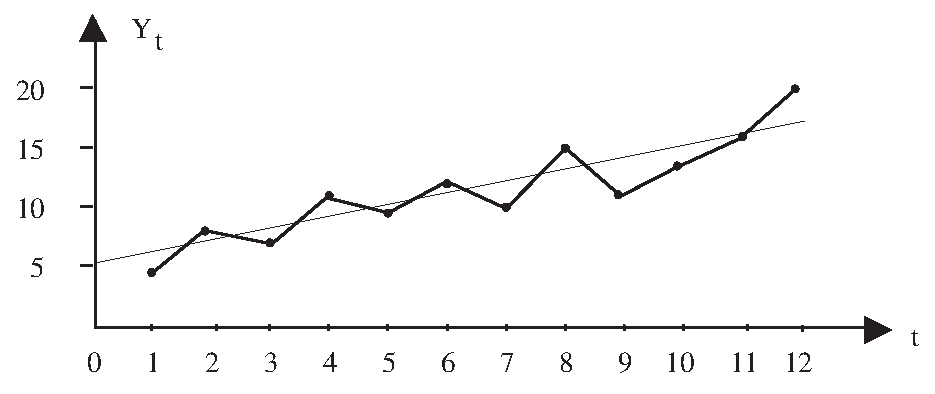
\includegraphics[scale=0.6]{figurer/fig13_1.pdf} 
 \caption{Tidsrekke med trend og sesongkomponent}
	\label{fig:sesong}
\end{figure}

Vi kan ha {\em periodiske variasjoner}, dvs. variasjoner som gjentar seg
med en viss regelmessighet etter et visst tidsrom.  Slike periodiske
varia\-sjoner kan bestå av korttidsvariasjoner og/eller langtidsvariasjoner.
Vi kjenner dette fra mange geofysiske tidsrekker, eksempelvis 
døgnvariasjoner og årvariasjoner, og fra økonomiske tidsrekker med
årlige sesongvariasjoner og/eller lengre konjunkturvariasjoner.  Det er
av og til nødvendig å skille ut konjunkturvariasjoner som er eget
element, bl.a. fordi slike ikke har en klart definert periodelengde i 
motsetning til rene sesongvariasjoner.

Det tredje element vi vil trekke fram er {\em autokorrelasjon}, dvs. en viss
avhengighet mellom etterfølgende verdier av tidsrekken.  Det er tale om
positiv autokorrelasjon som betyr at store (små) verdier 
gjennomgående etterfølges av store (små) verdier.  Det motsatte
er negativ autokorrelasjon som betyr at store (små) verdier 
gjennomgående etterfølges av små (store) verdier.  Et eksempel
på positiv autokorrelasjon vil være en periodedranker som etter
å ha drukket et stort kvantum den ene dagen, er tilbøyelig til å
følge opp den neste.  Mer seriøse eksempler finner vi i mange 
økonomiske tidsrekker hvor en påvirkning i en bestemt retning ofte
gjør seg gjeldende en tid framover.  Et eksempel på negativ 
autokorrelasjon kan være en fa\-mi\-lies daglige innkjøp av melk.  Det
finnes også økonomiske tidsrekker med slik karakter, typisk er 
innkjøpte kvanta for lager i etterfølgende perioder, etterspørsel
etter visse kostbare varer med et lite antall etterspørrere.

Det fjerde element som er typisk for tidsrekker er {\em tilfeldig variasjon},
dvs. variasjon som ikke kan forklares ut fra trend, periodisk variasjon
eller autokorrelasjon.

I praksis vil disse fire elementer kunne være til stede i varierende
grad, for noen tidsrekker kan enkelte elementer mangle helt.  Ved
tidsrekkeanalyse ønsker vi å klarlegge dette.  La oss illustrere noen
av disse forhold med figurer.

I Figur~\ref{fig:sesong} ser vi en tidsrekke som er observert kvartalsvis over tre år,
og observasjonene er representert ved punktene i figuren.  Her er det 
åpenbart en stigende trend, antydet ved den inntegnede rette linjen. Det er 
også en tydelig sesongkomponent med første kvartal som lavsesong og
fjerde kvartal som høysesong.  Om det i tillegg er autokorrelasjon er
vanskelig å si, trolig ikke.  La oss nå illustrere autokorrelasjon,
og for enkelhets skyld ser vi på tidsrekker uten trend og sesongvariasjon.
Tidsrekkene i Figurene~\ref{fig:autocor}a, \ref{fig:autocor}b og 
\ref{fig:autocor}c viser henholdsvis ingen, positiv og negativ
autokorrelasjon.

\begin{figure}[H]
   \centering
   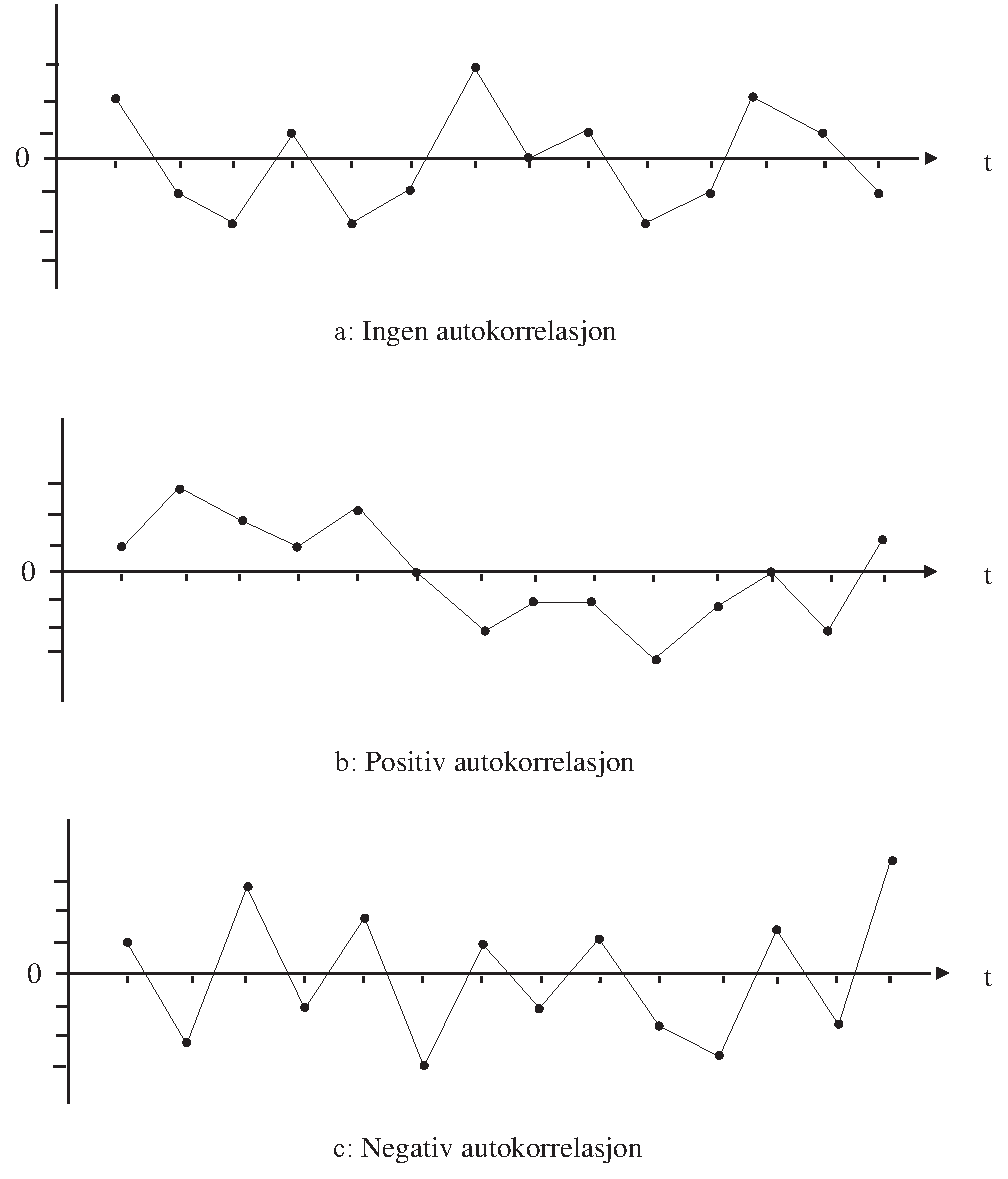
\includegraphics[scale=0.7]{figurer/fig13_2.pdf} 
   \caption{Ulik grad av autokorrelasjon}
	\label{fig:autocor}
\end{figure}

Vi er ofte interessert i en rask avklaring på om en tidsrekke uten trend og
sesong har autokorrelasjon eller ikke. En enkel test er den såkalte 
``run"-testen som tar utgangspunkt i om verdiene ligger på oversiden (+) 
eller undersiden ($-$) av ``nivået" til tidsrekken.
Antall ``følger" på hver side brukes som test\-observator,
se Oppgave~\ref*{kap:sannsynligheter_og_andeler}.37. Dette er moderat for ingen autokorrelasjon, 
mens det er lite (stort) for positiv (negativ) autokorrelasjon.  

For tidsrekkene i Figurene~\ref{fig:autocor}a--c er antall følger henholdsvis 10, 3 og 13.
Uavhengighet svarer til binomiske forsøk med $p=0.5$ for +,
og forventet antall følger og P-verdier kan dermed tilnærmet beregnes. 
En programvareutskrift av run-testen for den første tidsrekken 
(tallene er i Eksempel 5 nedenfor):

\begin{center} \framebox[10cm]{\begin{minipage}{9cm}\rule{0cm}{0.5cm}
\tt
>> runs 'rekke1' \\
 Expected no. of runs = 8\\
 Observed no. of runs =  10\\
 P-value = 0.2231  \\
 * note: n too small for good approximation \\

  \end{minipage}} \end{center}
Vi ser at antall runs ikke avviker mye fra forventet ved uavhengighet, og at
P-verdien ikke er spesielt liten, som støtter antakelsen om uavhengighet.
For de to andre tidsrekkene ble P-verdien ca. 0.006, dvs. klar indikasjon 
på avhengighet. 
Merk imidlertid at korte tidsrekker gir grove tilnærminger. \\[0.5cm]

\section{Analysemetoder}
La oss innføre følgende notasjon:  Vi betegner den observerte tidsrekken

\[  Y_1, Y_2, Y_3, \ldots, Y_n    \]

\noindent slik at $Y_t$ er den observerte verdi på tidspunkt $t$, og vi
antar her at vi har observert fram til og med tidspunkt $n$. Dersom vi skal
predikere tidsrekken videre framover i tiden, betegner vi prognosetallene
henholdsvis

\[ \hat{Y}_{n+1},\hat{Y}_{n+2},\hat{Y}_{n+3},\ldots \]

\noindent slik at $\hat{Y_t}$ betegner predikert verdi av tidsrekken for
tidspunkt $t$.

Det er vanskelig å lage en generell teori for analyse av
tidsrekker som er egnet under alle omstendigheter. Det finnes derfor flere 
angrepsmåter som hver kan ha sine fortrinn under ulike forhold, men som
også i noen grad konkurrerer om brukerens gunst.  Det vil derfor være
et spørsmål om valg på grunnlag av den innsikt som brukeren har 
om det foreliggende problem og de forhold som ønskes belyst.


Vi vil først ta opp analyse av tidsrekker der trend og sesongvariasjoner
er de dominerende trekk.  Dette vil ofte være tilfellet for mange
tidsrekker i økonomiske sammenhenger, hvor sesongkomponenten kan bestå
i varia\-sjoner med årstiden for månedlige eller kvartalsvise data, eller 
variasjoner med ukedag for daglige data.  Vi vil for enkelhets skyld anta at det
bare er en sesongkomponent som gjentar seg periodisk, eksempelvis fra år
til år.  Et eksempel på en slik tidsrekke har vi i Figur~\ref{fig:sesong}, hvor en
tidsrekke er observert kvartalsvis over tre år.  Vi vil foreløpig
holde autokorrelasjon utenfor i diskusjonen, men kommer tilbake til dette
senere.

Vi vil først ta for oss en meget enkel metode for analyse av tidsrekker
med trend og sesongvariasjoner.  Metoden bygger på følgende modell

\[     Y=T \cdot S \cdot U .  \]

\noindent Vi tenker oss altså hver tidsrekkeverdi $Y$ som et produkt av en 
trendverdi $T$, en sesongfaktor $S$ og en tilfeldig faktor $U$ som skyldes
andre omstendigheter.  Dersom vi på grunnlag av den observerte tidsrekken
$Y_1, Y_2, \ldots, Y_n$ har fastlagt de tilhørende $T_t, S_t, U_t$ for
$t = 1, 2, \ldots, n$, sier vi at vi har dekomponert tidsrekken.  Ved en slik
dekomponering vil trenden $T$ angis med den samme enhet som tidsrekken selv,
mens sesongfaktoren $S$ og den tilfeldige faktor $U$ oppfattes som indekser
som gir det prosentvise avvik fra trenden.  Disse indeksene bør 
følgelig variere omkring 1 over tid.  Sesongindeksen skal gi uttrykk for
periodiske avvik, og gis derfor verdier som gjentar seg fra periode til
periode.\\

\begin{eksempel}{Fyringsolje}
En leverandør av fyringsolje har de siste 5 1/2 år notert
månedlig salg $Y_1,Y_2,\ldots, Y_{66}$.  Tidsrekken (ikke vist her)
har en klar trend og sesong\-varia\-sjoner med en periode på 12 måneder. I
desember i fjor (måned nr.60) ble det solgt $Y_{60} $ = 224 000 liter. 
Ifølge den trend som synes å foreligge ``burde" de ha solgt
$T_{60}$ = 200 000 liter.  Nå er desember høysesong og en analyse viser
at desembersalget gjennomgående er 40\% over den generelle trenden, vi
setter  $S_{12} = S_{24}=\cdots = S_{60} = 1.40$. 
Nå var tilfeldigvis desember måned spesielt 
mild dette året og en regner at dette medførte at desembersalget 
dette året var 20\% lavere enn vanlig, svarende til $U_{60} = 0.80$.
Vi har dermed fått skrevet $Y_{60} = T_{60} \cdot S_{60} \cdot U_{60}$.
\end{eksempel}

Alternativt kunne en tenke seg å dekomponere tidsrekken ut fra en
lineær modell

\[     Y = T + S + U    \]

\noindent Her blir alle størrelser målt med de samme enheter, $S$ og
$U$ gir da uttrykk for absolutte og ikke prosentavvik fra trenden $T$. 
Både $S$ og $U$ bør variere omkring null, den første periodisk.

De to modellene er beslektet, idet den første modellen $Y = T \cdot S 
\cdot U$ alternativt kan skrives

\[ logY=logT+logS+logU \]

\noindent slik at denne modellen svarer til en lineær dekomposisjon for 
logaritmen til de opprinnelige størrelsene.  Den første modellen er 
først og fremst aktuell i situasjoner der sesongutslagene er 
gjennomgående proporsjonale med trendens verdi, mens den lineære
modellen er aktuell når sesongutslagene gjennomgående ikke avhenger
av trendens verdi.

Uansett hvilken dekomponeringsmodell som velges vil det første trinn i
analysen som regel være å fastlegge trenden.  Dette kan gjøres ved
ulike metoder.  I mange situasjoner er det rimelig å prøve å
tilpasse en lineær trend, dvs. betrakte trenden som en lineær
funksjon av tiden.  Ut fra et plott av tidsrekken kan vi, etter beste 
skjønn, tegne inn en rett linje som angir hovedtendensen.  Mer vanlig er 
å bestemme minste kvadraters regresjonslinje for $Y$ med hensyn på
tiden $t$, dvs. at trenden blir bestemt ved

\[    T = \hat{\gamma} + \hat{\beta} \cdot t  \]

\noindent der $\hat{\gamma}$ og $\hat{\beta}$ er fastlagt ved minste
kvadraters metode, se Kapittel 8.3. Trenden er da stigende eller synkende alt
ettersom $\hat{\beta}$ blir positiv eller negativ. En $\hat{\beta}$ nær null
svarer til at det ikke er noen langtidsutvikling i tidsrekken, i hvert fall
ikke lineær.

Enkelte tidsrekker kan ha et utviklingsforløp som ikke er forenlig med
en lineær trend, det kan da være aktuelt å bruke andre 
funksjonsformer, og en rekke slike er studert i litteraturen, eksponensiell
vekst osv.  I praksis vil det som regel være lite å hente ved å
forlate tanken om lineær trend med mindre dette er åpenbart 
urealistisk, enten vurdert ut fra den foreliggende tidsrekken eller ut fra
allment aksepterte teorier som er relevante for det foreliggende problem.

Det å bestemme langtidsutviklingen i en tidsrekke kan også oppfattes
som å glatte tidsrekken, dvs. fjerne uregelmessigheter, som ifølge
vår mo\-dell har karakter av sesongavvik og tilfeldige avvik fra en trend.
Det finnes en rekke metoder for glatting av tidsrekker, en av disse er
såkalte {\em glidende gjennomsnitt}.\\

\begin{eksempel}{Glidende gjennomsnitt}
Betrakt følgende utsnitt av en tidsrekke
\begin{center}
\begin{tabular}{lcccccccccc}
Tidsrekke:    & $\cdots$ & 2 & 6 & 1 & 5 & 6 & 4 & 5 & 9 & $\cdots$ \\
Glidende gjennomsnitt: & & $\cdots$ & 3 & 4 & 4 & 5 & 5 & 6 &$\cdots$ &
\end{tabular}
\end{center}
Her er beregnet gjennomsnitt av orden 3, dvs. hvert tall i annen linje er 
gjennomsnittet av de tre nærmeste tall i linjen over.  Vi ser  at den nye
rekken er en glattet versjon av den første, og gir dermed et uttrykk for
hovedtendensen for øyeblikket, som her er stigende.
I forbindelse med tids\-rekker som 
observeres månedlig med sesongvariasjoner over 12 måneder, er det
aktuelt å beregne glidende gjennomsnitt av orden 12.  På dette viset
blir sesongvariasjonene og tilfeldige variasjoner i rekken i noen grad glattet
ut og det som gjenstår er i hovedsak trend.  Dersom tidsrekken 
observeres kvartalsvis, vil glidende gjennomsnitt av orden 4 kunne brukes.
\end{eksempel}

Glidende gjennomsnitt blir ofte brukt i situasjoner hvor vi ikke på
forhånd har bestemte forestillinger om langtidsutviklingen.  Ofte kan en
slik analyse peke i retning av en lineær trend eller en annen klar trend,
i så fall bør dette følges opp \footnote{Det knytter seg også
visse reservasjoner til bruk av glidende gjennomsnitt.  En avvikende
observasjon kan forårsake at den nye rekke får en bølgefasong som
ikke er til stede i den opprinnelige rekke, såkalt Slutsky-Yule effekt.}.
Imidlertid kan det også hende at slik ana\-lyse ikke avdekker noen klar 
trend og det er da ofte urimelig å fortsette etter den modell vi startet 
med.  Det er da trolig andre trekk enn trend og sesongvariasjoner som er 
særmerkt ved tidsrekken og dette vil kreve en annen modell og andre 
metoder.

Vi vil i det følgende anta at vi har valgt å dekomponere
en tidsrekke etter modellen $Y = T \cdot S \cdot U$.  La oss tenke oss at
trenden er fastlagt på grunnlag av tidsrekken $Y_1, Y_2, \ldots, Y_n$, ut
fra de metoder som er skissert ovenfor eller på annen måte.  La oss
betegne den fastlagte trend med $T_t$.  Vi kan da beregne $Z_t = Y_t/T_t$;
$t = 1, 2, \ldots, n$.  Ifølge modellen kan vi skrive $Z_t =S_t\cdot U_t$,
 dvs. $Z_t$ kan oppfattes som en tidsrekke der trenden er fjernet, men
der sesongvariasjoner og tilfeldige variasjoner fortsatt er til stede.  Vi
ønsker nå å bestemme sesongindekser, og dette kan skje ved å
fjerne de tilfeldige variasjonene i tidsrekken $Z_t$.

La oss for enkelhets skyld anta at tidsrekken består av månedlige
data med sesongvariasjoner over 12 måneder.  Vi kan da ta for oss 
verdiene av $Z_t$, svarende til samme måned i alle de år som
tidsrekken omfatter.  Tar vi gjennomsnittet av disse tallene vil 
tilfeldigheter fra år til år reduseres og dette gjennomsnittet tas
da som sesongindeks for vedkommende måned.  Vi får da bestemt 12
sesongindekser $S_1, S_2,\ldots, S_{12}$ som gir uttrykk for sesongvariasjonen
uansett år, slik at
 $S_1 = S_{13} = S_{25} = \cdots, S_2 = S_{14} = S_{26}= \cdots,
\cdots, S_{12} = S_{24} =S_{36} = \cdots$.  Disse blir ofte justert slik at
gjennomsnittet over en periode er lik 1. Vi kan nå beregne $U_t = Z_t/S_t$
 for $t = 1, 2, \cdots, n$, som gir uttrykk for de tilfeldig avvik fra 
måned til måned.

Vi ser at vi kan gjennomføre en helt analog analyse på grunnlag av
den lineære modellen $Y_t = T_t + S_t + U_t$, idet vi etter tur trekker
fra de størrelser som er fastlagt istedenfor å dividere.

På grunnlag av en dekomponert tidsrekke $Y_t = T_t \cdot S_t \cdot U_t$
er det naturlig å bruke følgende prediktor for framtidige verdier

\[ \hat{Y}_t=T_t \cdot S_t \mbox{\ \ \ \ } t=n+1,n+2, \ldots  \]

\noindent Den trend som ble observert i tidsrommet $t = 1,2,\ldots, n$
forlenges ut i framtida, og samme sesongindeks brukes.  Indeksen for
tilfeldige avvik er satt lik 1 da vi ikke kan forutsi disse.
Dersom vår analyse var basert på den lineære modellen,
ville vi sette $\hat{Y_t} = T_t + S_t$.\\

\begin{eksempel}{Dekomponering}
En tidsrekke $Y_t$ er observert kvartalsvis i en treårsperiode, dvs. for
$t = 1, 2, \ldots, 12$, og det er denne tidsrekken som er illustrert i Figur~\ref{fig:sesong}
ovenfor.  La oss utføre en analyse basert på dekomponering av form
$Y = T \cdot S \cdot U$.  På øyemål ser det ut til at trenden er
lineær, og kan la seg tilfredsstillende representere ved $T_t = 5 + 1
\cdot t$.  Minste kvadraters metode gir imidlertid $T_t = 4.4 + 1.1 \cdot t$,
og dette er brukt i beregningene i tabellen nedenfor.
Med denne dekomponering predikeres tidsrekkens verdi for
første kvartal kommende år:
\[ \hat{Y}_{13}=T_{13} \cdot S_{13}=(4.4+1.1 \cdot 13) \cdot 0.82=15.3   \]
\noindent og for fjerde kvartal kommende år
\[ \hat{Y}_{16}=T_{16} \cdot S_{16}=(4.4+1.1 \cdot 16) \cdot 1.19=26.2  \] 
%\begin{center}
\begin{tabular}{|rr|rrrr|} \hline
 $t$ &   $Y_t$    &     $T_t$   &    $Z_t$   &     $S_t$  &   $U_t$  \\ \hline
  1  &    4.8     &      5.5    &     0.87   &     0.82   &     1.06   \\
  2  &    7.7     &      6.6    &     1.17   &     1.05   &     1.11   \\
  3  &    7.2     &      7.7    &     0.94   &     0.94   &     1.00   \\
  4  &   10.8     &      8.8    &     1.23   &     1.19   &     1.03   \\
  5  &    8.0     &      9.9    &     0.81   &     0.82   &     0.99   \\
  6  &   12.1     &     11.0    &     1.10   &     1.05   &     1.05   \\
  7  &   10.8     &     12.1    &     0.89   &     0.94   &     0.95   \\
  8  &   15.6     &     13.2    &     1.18   &     1.19   &     1.00   \\
  9  &   11.2     &     14.3    &     0.78   &     0.82   &     0.95   \\
 10  &   13.5     &     15.4    &     0.88   &     1.05   &     0.84   \\
 11  &   16.0     &     16.5    &     0.97   &     0.94   &     1.03   \\
 12  &   20.4     &     17.6    &     1.16   &     1.19   &     0.97 \\ \hline
\end{tabular} 
%\end{center}
\end{eksempel}
Ved denne form for analyse er det ikke lett å vurdere
påliteligheten i eventuelle konklusjoner.  Til det kreves ytterligere
forutsetninger om de størrelser som inngår i modellen. 
Slike forutsetninger kan også sette
oss i stand til å vurdere egenskapene ved den foreslåtte 
prognosemetode kontra andre metoder.

En alternativ framgangsmåte for analyse av trend og sesongvariasjon er 
å ta utgangspunkt i en lineær regresjonsmodell.\\


\begin{eksempel}{Omsetning}
En bedrift registrerer kvartalsvise omsetningstall og regner med en lineær
trend og at fjerde kvartal er høysesong i forhold til de tre første 
kvartalene.  Følgende modell er da aktuell

\[  Y={\beta}_0+{\beta}_1 t + {\beta}_2 Q + U \]

\noindent der $t$ betegner tidspunkt og $Q$ er en indikatorvariabel som er 1
dersom observasjonen svarer til fjerde kvartal og $0$ ellers, og $U$ er
tilfeldig avvik.  Parametrene ${\beta}_0, {\beta}_1$ og ${\beta}_2$ er ukjente
og ønskes fastlagt på grunnlag av den observerte tidsrekke.  Modellen 
ovenfor kan bygges ut i ulike retninger, til trender som ikke er lineære i
tid, og til mer enn to sesongtyper.  Det siste kan skje ved å innføre
flere sesongvariable.  La oss bruke en modell av denne typen på 
problemstillingen i Eksempel 3, hvor trolig alle fire kvartaler er ulike.
Modellen blir da

\[ Y={\beta}_0+{\beta}_1 t + {\beta}_2 Q_2 + {\beta}_3 Q_3
                            + {\beta}_4 Q_4 + U \]

\noindent der $Q_i$ er 1 dersom observasjonen svarer til i'te kvartal og 0
ellers for $i = 2, 3, 4$. Merk at det er nok med tre indikatorvariable for
å beskrive forskjeller for de fire kvartalene.  La oss bruke tallmaterialet
til å bestemme koeffisientene ved minste kvadraters metode, betegn
disse med $\hat{{\beta}_0}, \hat{{\beta}_1}, \ldots, \hat{{\beta}_4}$ (se
Kapittel 12.2).  Som prediktor brukes 

\[  {\hat{Y}}_t={\hat{\beta}}_0+{\hat{\beta}}_1 t + {\hat{\beta}}_2 Q_2
                            + {\hat{\beta}}_3 Q_3 + {\hat{\beta}}_4 Q_4 . \]
\noindent Våre observasjoner gir

\[ {\hat{Y}}_t=3.22+0.96\cdot t + 2.14 \cdot Q_2 + 1.42 \cdot Q_3
                                                 + 4.73 \cdot Q_4   \]
\noindent som bl. a. gir følgende prognoser
\begin{eqnarray*}
 {\hat{Y}}_{13}&=&3.22+0.96\cdot 13 + 2.14 \cdot 0 + 1.42 \cdot 0 
                                                 + 4.73 \cdot 0 = 15.7 \\
 {\hat{Y}}_{16}&=&3.22+0.96\cdot 16 + 2.14 \cdot 0 + 1.42 \cdot 0 
                                                 + 4.73 \cdot 1 = 23.3
\end{eqnarray*}
\end{eksempel}
Sesongvariasjoner har ofte en syklisk karakter i den forstand at i løpet
av sesongperioden vil sesongeffekten gå gradvis fra f.eks. lavsesong,
via middels sesong til høysesong, deretter via middels sesong til 
lavsesong igjen ved starten av neste sesongperiode.  Det er mulig å lage
modeller hvor en tar omsyn til dette, og dermed får ytterligere forbedret
eventuelle prognoser.  Tidsrekken i Eksempel 3 ser imidlertid ut til å
ikke ha denne karakter, høysesong etterfølges direkte av lavsesong.

Fordelen med en analyse basert på en lineær regresjonsmodell, der alle
elementene trend, sesongavhengighet og tilfeldig variasjon kommer til uttrykk,
er at vi kan støtte oss på en velutviklet teori, se Kapittel 12.
Betraktes de variable som inngår i modellen som stokastiske variable med 
nærmere angitte egenskaper, kan vi komme
med presise utsagn om trenden og sesongvariablenes betydning, usikkerheten
ved prediksjoner osv.  Med tilgang til god programvare vil man som
regel foretrekke en analyse basert på en regresjonsmodell framfor den mer
klassiske analysen presentert ovenfor.


For analyse og prediksjon av tidsrekker i praksis trengs metoder som også 
kan ta omsyn til autokorrelasjon og andre spesielle særtrekk,
herunder såkalt ikke-sta\-sjo\-næ\-ritet, som ofte
forekommer i økonomiske data. I litteraturen fins flere hovedretninger,
og vi nevner (med populær metode i parentes):
\begin{itemize}
\item  ``Time Series Analysis and Prediction'' (Box-Jenkins metode)
\item ``Time Series Forecasting'' (Holt-Winter's metode)
\end{itemize}
Box-Jenkins metode er knyttet til den såkalte generelle ARIMA-modellen,
mens Holt-Winters metode er mindre generell, men legger i steden vekt
på et mer fleksibelt system for oppdatering av prognoser etterhvert som 
nye data kommer til. 

Det fins idag et rikelig tilbud på brukervennlig programvare for
tids\-rekke\-analyse og prediksjon, men det er vanskelig å gi generelle
 anbefalinger om metode. En advarsel mot bruk av tilsynelatende
avanserte metoder som er automatiserte, med få krav til brukeren,
er imidlertid på sin plass. Det lønner seg som regel å
holde seg nær til dataene.
Et problem i praksis er hvor lang tidsrekke som trengs for å bruke
metoden med en viss trygghet. For en del avanserte metoder trengs gjerne
mer enn 50 observasjoner, men da møter en raskt problemet at
omstendighetene er endret fra de første til de siste observasjonene.

Selv om vi her ikke vil gjennomgå noe avansert system for
analyse og prediksjon av tidsrekker, vil vi bruke den enkle
dekomponeringsmodellen til å forklare hvordan slike systemer i prinsippet
kan ta omsyn til trend, sesongvariasjon og autokorrelasjon.

Først søker en å bestemme trenden og sesongvariasjonene og fjerne 
disse fra tidsrekken, slik at vi sitter igjen med en rekke hvor 
autokorrelasjon er det dominerende trekk.  På denne rekken kan vi anvende
tilgjengelige metoder for analyse av autokorrelasjonen. Når de tre 
elementene trend, sesongavhengighet og autokorrelasjon er isolert, kan de 
igjen kombineres til å gi prediksjoner av framtidige verdier av tidsrekken
som tar hensyn til alle tre særtrekk ved rekken.

Anta vi har en tidsrekke som vi har valgt å dekomponere i henhold til
den lineære modellen $Y_t = T_1 + S_t + U_t$.  Anta at en lineær
trend $\hat{T_t}$ og sesongkomponenter $\hat{S_t}$ er fastlagt ut fra den
observerte rekke, slik at beregnede verdier er $\hat{Y_t} = \hat{T_t} +
\hat{S_t}$.  De beregnede feilledd er da $\hat{U_t} = Y_t - \hat{Y_t}$.  La
oss illustrere de prinsipielle sider ved figurer.

I Figur~\ref{fig:trend_sesong}a er den lineære trenden $\hat{T_t}$ videreført ut over den
observerte rekke til framtid, og i Figur~\ref{fig:trend_sesong}b er sesongkomponenten $\hat{S_t}$
videreført.  Resi\-dualene $\hat{U_t}$ i Figur~\ref{fig:trend_sesong}c viser tydelig tendens til
negativ autokorrelasjon og denne tendens er videreført et kort stykke ut
i fremtid.  Den prognose som gis for fremtidige $t$ er dermed gitt ved
${\hat{Y}}_t={\hat{T}}_t+{\hat{S}}_t+{\hat{U}}_t, t=n+1,n+2, \ldots $

\begin{figure}[H]
\centering
   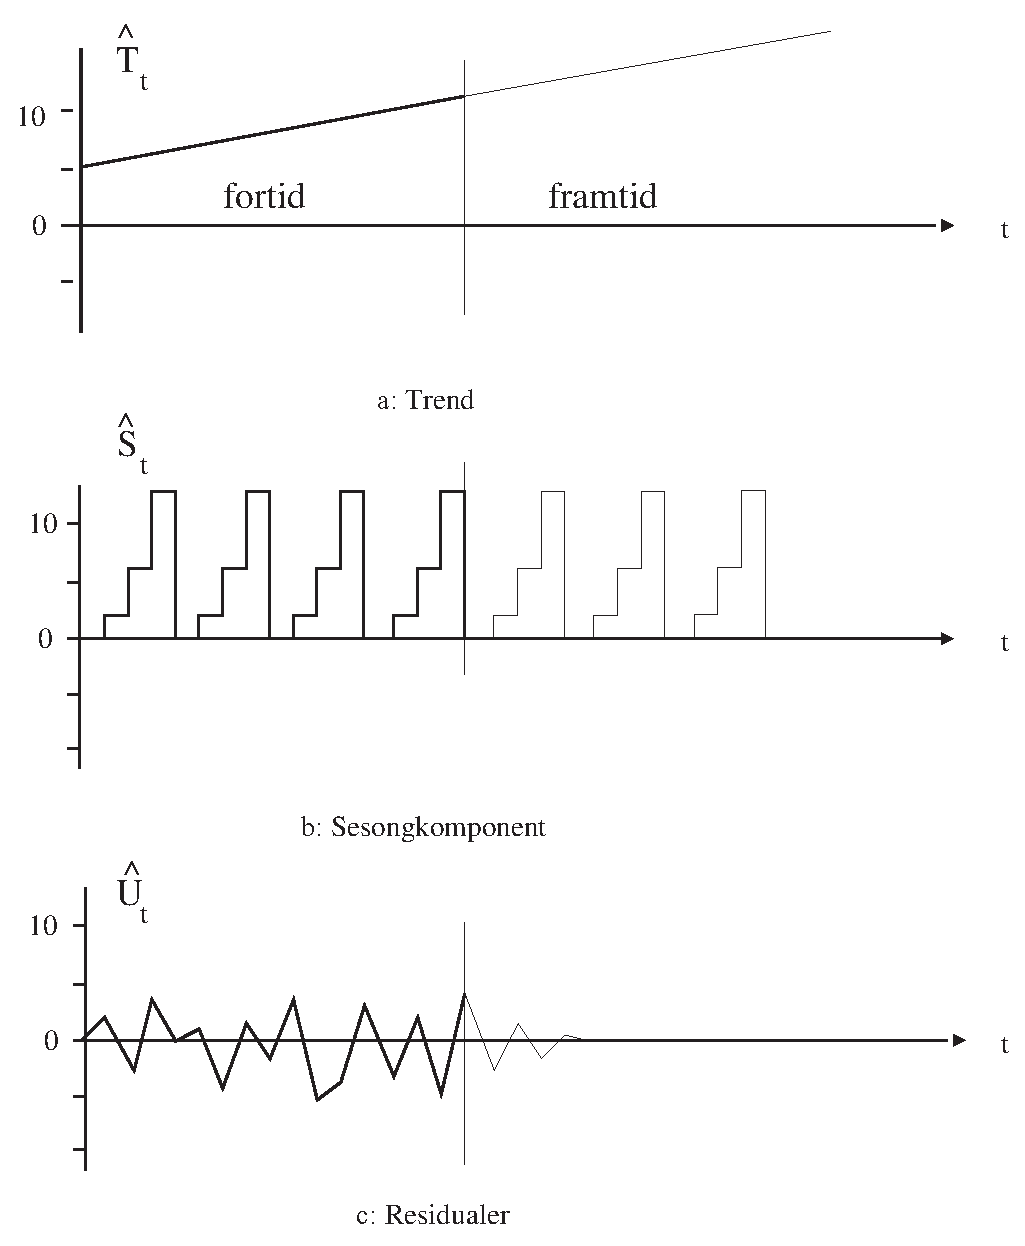
\includegraphics[scale=0.6]{figurer/fig13_5.pdf} 
   \caption{Trend og sesong i tidsrekke}
	\label{fig:trend_sesong}
\end{figure}

\section{Autokorrelasjon}
Vi vil i dette avsnittet ta for oss sentrale begreper knyttet til 
autokorrelasjon, og noen sentrale tidsrekkemodeller for autokorrelasjon.
Disse er aktuelle  for analyser og prognoser i praksis, og er
også et godt utgangspunkt for videre studier dersom situasjonen krever
andre metoder.


Autokorrelasjon kan opptre sammen med trend og/eller sesongvariasjon, men la
oss i første omgang anta at slike elementer ikke er til stede, slik at
tidsrekken i hovedsak kan ha karakter som illustrert før i Figurene~\ref{fig:autocor}a--c.

La $Y_t$; $t=1,2,\ldots n$ være en tidsrekke, der $Y_t$'ene
oppfattes som sto\-kas\-tiske variable med samme forventning $\mu $ og varians
${\sigma}^2$, men der det er tidsavhengighet.  Et teoretisk mål for denne
tidsavhengigheten er gitt ved den såkalte {\em autokovariansfunksjonen}

\[  c_t(k)=cov(Y_t,Y_{t+k})      \]

\noindent Spesielt interessant er denne størrelsen dersom tidsrekken er
{\em stasjonær}, som grovt sagt betyr at karakteren av rekken er den samme
uansett hvilken tidsperiode vi betrakter.  Autokovariansen avhenger da ikke 
av $t$, men bare av forskjellen i tid mellom de to tidspunktene i formelen,
og vi skriver da $c(k)$. Merk at $c(0) = {\sigma}^2$.  For å skaffe 
innsikt i tidsavhengigheten er det aktuelt å anslå denne 
autokovariansen ut fra den observerte rekke $Y_1, Y_2, \ldots, Y_n$, f.eks.
ved 

\[ \hat{c}(k)=\frac{1}{n-k} \sum_{t=1}^{n-k} (Y_t-\bar{Y})(Y_{t+k}-\bar{Y}) . \]
Et nærmere studium av den estimerte autokovariansfunksjonen kan
bidra til konstruksjon av en brukbar modell for tidsavhengighet i rekken.
Mer praktisk er å studere estimatet for den tilhørende
 {\em autokorrelasjonsfunksjonen}
          \[ r(k)=c(k)/c(0).  \]
Det finnes en rekke metoder for tidsrekkeanalyse som bygger på
forutsetningen om at tidsrekken er stasjonær. La oss presentere to
enkle  modeller av dette slaget, som også kan vise vei til mer kompliserte
modeller. Først
\[ Y_t= \gamma +\rho Y_{t-1} + U_t       \]
I denne modellen oppfattes tidsrekkens verdi på tidspunkt $t$
som en lineær funksjon av dens verdi på tidspunkt $t - 1$ pluss et
feilledd som uttrykker en tilfeldig påvirkning på tidspunkt $t$. Vi
vil anta at disse feilleddene er uavhengige stokastiske variable med
forventning null og samme varians.  Parameteren $\rho$  uttrykker graden av
autokorrelasjon og må i praksis være et tall mellom $-1$ og $+1$,
ellers vil tidsrekkens verdier kunne vokse over alle grenser:  Positiv $\rho$
uttrykker positiv autokorrelasjon, negativ $\rho$ uttrykker negativ
autokorrelasjon. Uavhengighet svarer til $\rho =0$.
Denne modellen kalles {\em autoregresjon av første orden}, og benevnes
AR(1). Mer generelt vil en AR(p) modell  uttrykke $Y_t$ ved verdier
$1,2,\ldots ,p$ tidsenheter bakover i tid. En annen type modell er

\[ Y_t= \mu +\alpha U_{t-1} + U_t       \]
Her oppfattes tidsrekkens verdi på tidspunkt $t$ som en lineær 
funksjon av tilfeldige påvirkninger på tidspunkt $t$ og ett trinn
bakover i tid. Disse antas uavhengige stokastiske variable med
forventning null og samme varians.  Parameteren $\alpha$ uttrykker graden av
avhengighet med forrige tidspunkt.
Denne modellen kalles ofte {\em bevegelig gjennomsnitt (``moving average'')
av første orden}, og benevnes MA(1). Mer generelt vil en MA(q) modell 
 uttrykke $Y_t$ ved tilfeldige påvirkninger $0,1,2,\ldots ,q$ tidsenheter
bakover i tid.
Disse to modelltyper kan kombineres til den såkalte ARMA(p,q) modellen.

Merk at tilfellet med uavhengige observasjoner, ofte kalt {\em ren støy}
(PN for ``pure noise"), fremkommer som spesialtilfeller av AR(1) og MA(1) ved å sette hhv. 
$\rho=0$ og $\alpha=0$. En annen interessant tidsrekkemodell er såkalt
\emph{``random walk"}(RW) gitt ved
\[ Y_t = Y_{t-1} + U_t       \]
som er grensetilfellet for AR(1) når $\rho=1$. Her er endringene ``ren
støy". 

For AR(1) og MA(1) modeller vil autokorrelasjonsfunksjonen ha en enkel form,
som gjør at tidsrekker av dette slaget er forholdsvis enkle å
identifisere. Vi har nemlig (se Oppgave~11 og~12):
\begin{center}
\begin{tabular}{ll}
Modell & Autokorrelasjonsfunksjon \\ \hline
PN     & $r(k)=0$ for $k>0$  \\
MA(1)  & $r(1)\neq 0$, $r(k)=0$ for $k>1$  \\
AR(1)  & $r(k)={\rho}^k$ for $k>0$  \\ \hline                              
\end{tabular}
\end{center}
For identifikasjon i praksis ser en på et såkalt ACF-plott, med estimater for
$r(k)$ som funksjon av $k$, beregnet på grunnlag av den observerte 
tidsrekke, og som det derfor hefter usikkerhet ved.
Et plott med små autokorrelasjoner uten klart mønster sannsynliggjør
PN som modell, en klar ``pigg" for $k=1$ og ellers intet mønster 
indikerer MA(1), mens et eksponensielt avtagende mønster indikerer AR(1).
For identifikasjon av mer kompliserte modeller trenger en ytterligere kjennetegn
som vi ikke skal gå inn på her.

Typisk for stasjonære tidsrekker er at autokorrelasjonen avtar 
forholdsvis raskt mot null. Dette er ikke tilfellet for en ``random walk".
En slik kan imidlertig identifiseres ved å sjekke om differensene er
``ren støy".\\

\begin{eksempel}{Autokorrelasjon}
Betrakt de tre tidsrekkene i Figur~\ref{fig:autocor}a--c.  Disse er: 
\begin{center}
\begin{tabular}{lrrrrrrrrrrrrrr}
 $Y_t$:     & 2&-1&-2&  1&-2&-1&  3&  0&  1& -2&-1&  2&  1&-1 \\
 $Y^{'}_t$: & 1& 3& 2&  1& 2& 0& -2& -1& -1& -3&-1&  0& -2& 1 \\
 $Y^{''}_t$:& 1&-2& 3& -1& 2&-3&  1& -1&  1& -2&-3&  2& -2& 4
\end{tabular}
\end{center}
Et ACF-plott av så korte rekker som dette gir ikke god mening i praksis,
men hvis noe antyder et slikt at den første rekken ikke
har klar auto\-korrelasjon, mens den andre og tredje rekken har henholdsvis
positiv og negativ autokorrelasjon, med AR(1) som aktuell modell.
Et mer realistisk eksempel kommer til slutt i avsnittet.
\end{eksempel}


Når en egnet modelltype er identifisert, vil den som regel inneholde
ukjente parametre som må estimeres ut fra tidsrekken.
Dersom vi har valgt en AR(1) modell, kan vi estimere $\rho$ med
minste kvadraters estimatoren 

\[ \hat{\rho} = \frac{\sum_{t=2}^{n}Y_{t-1}Y_t}{\sum_{t=1}^{n}Y_t^2} \]
Formelen forutsetter (som i eksemplet) at gjennomsnittsnivået er null, se
Oppgave~\ref*{kap:regresjonsanalyse}.13 og~\ref*{kap:regresjonsanalyse}.15.

Generelt vil estimering av ukjente parametre i ARMA-modeller være relativt
komplisert, og en trenger programvare for beregningene.\\

\begin{eksempel}{Autoregresjon}
La oss estimere $\rho$ for AR(1) modell for de tre tidsrekkene i Eksempel 5.
Vi får henholdsvis

\[ \rho =-0.17 \mbox{\ \ \ }{\rho}^{'}=0.50 \mbox{\ \ \ }{\rho}^{''}=-0.56 \]

\noindent Den første rekken har en negativ estimert koeffisient, men ikke 
tilstrekkelig negativ til å forlate antakelsen om uavhengighet.  
Koeffisientene for de to andre rekkene er i samsvar med det vi ventet oss,
henholdsvis klar positiv og klar negativ autokorrelasjon.
\end{eksempel}

La oss kort se hvordan en kunne predikere en AR(1) tidsrekke (anta for
enkelhets skyld at forventningen er null):
Med observert tidsrekke $Y_1, Y_2, \ldots, Y_n$ vil vi,
dersom $\rho$ var kjent, predikere den neste verdi av tids\-rekken slik

\[   {\hat{Y}}_{n+1}=\rho Y_n      \]
Det tilhørende feilledd kan ikke forutsies ut fra tidsrekken, og
blir følgelig erstattet med sin forventning null.  Vi ser at for positiv
autokorrelasjon har prognosen samme fortegn som den sist observerte verdien,
men i tall\-verdi noe mindre enn denne.  Ved negativ autokorrelasjon skifter
prognosen fortegn i forhold til den sist observerte verdi.  Legg merke til at 
med en første ordens modell har vi ingenting å hente ved å ta 
omsyn til enda tidligere verdier av tidsrekken.  En prognose for tidsrekkens 
verdi $k$ tidsenheter senere vil være (Oppgave~13)

\[   {\hat{Y}}_{n+k}={\rho}^k Y_n    \]

\noindent Vi ser at når $k$ vokser vil prognosen nærme seg null, som
er rimelig fordi et stykke ut i tid vil de tilfeldige variasjonene gjøre
seg såpass gjeldende at det er risikabelt å være mer spesifikk.\\

\begin{eksempel}{Prognose}
Anta at de tre tidsrekkene i Eksempel 5 er observert over en lengre periode 
som går forut for de 14 observasjonene som er gitt i eksemplet og at
en på dette grunnlag har bestemt seg for en AR(1)
modell med parameter $\rho$ henholdsvis 0.0, 0.6 og -0.6.
Prognosen fra tidspunkt 2 og et skritt framover blir for de tre rekkene
henholdsvis 0.0, 1.8 og 1.2, mens de faktisk observerte verdier ble
henholdsvis -2, 2 og 3. 
\end{eksempel}

Dersom parameteren $\rho$ ikke er kjent, men  estimert lik $\hat{\rho}$ ut
fra tids\-rekken, kan vi bruke prediktorer av formen ovenfor, hvor $\rho$ er
erstattet med $\hat{\rho}$. Dersom tidsrekken varierer om et nivå ulik
null, korrigeres formlene med det beregnede gjennomsnitt av tids\-rekken.

Generelt vil prognoseformler i ARMA-modeller være relativt
kompli\-serte, og en trenger programvare for beregningene.\\

\begin{eksempel}{Identifikasjon}
La oss studere nærmere tidsrekken gitt i Oppgave~\ref*{kap:introduksjon}.13. 
Den ser slik ut:

\begin{figure}[ht]
\centering
   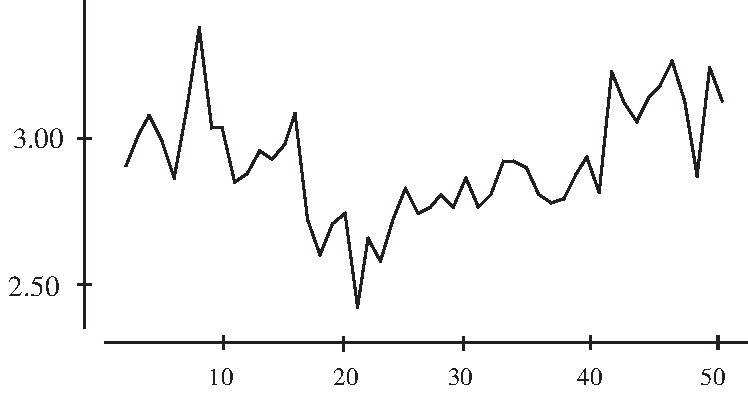
\includegraphics[scale=0.8]{figurer/fig13_8.pdf} 
 \caption{Tidsrekke med autokorrelasjon}
	\label{fig:tidsrekke_acf}
\end{figure}

\noindent
Den ligner det vi ofte ser for kurser på børsnoterte aksjer.
Et ACF-plott viser at autokorrelasjonene avtar sent mot null, noe som tyder
på at rekken ikke er stasjonær, men at endringene fra et tidspunkt
til det neste kan være det. ACF-plottet for disse ser slik ut:

\begin{figure}[ht]
\centering
   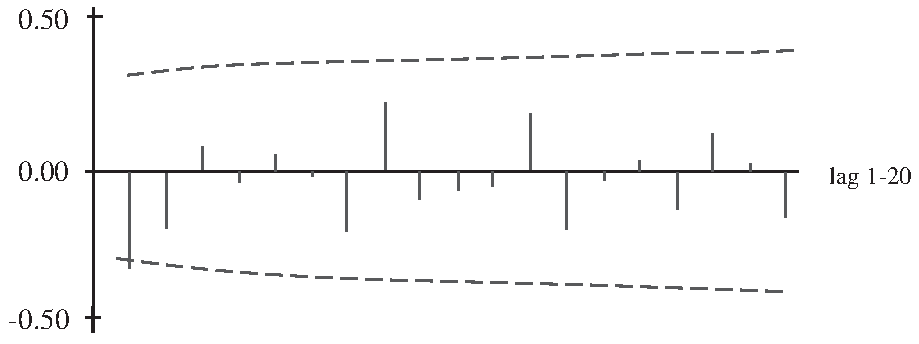
\includegraphics[scale=0.7]{figurer/fig13_9.pdf} 
 \caption{Autokorrelasjonsfunksjon (estimert)}
	\label{fig:}
\end{figure}

"Piggen" ved ``lagg" k=1 ligger på grensen til å være signifikant
(95\% konfidensgrenser er stiplet i figuren), mens de øvrige pigger ikke
tillegges betydning. Aktuelle modeller for differensene er derfor
PN eller MA(1). Det er naturlig å forsøke det siste, og etter
estimering av modellen teste om MA-parameteren er statistisk signifikant.
Dette er en såkalt ARIMA(0,1,1) modell. Her er en programvareutskrift:
\begin{center} \framebox[10cm]{\begin{minipage}{9cm}\rule[-0.5cm]{0cm}{0.5cm}
\tt 

 >> READ 'oppg1.13' 'data'\\
 >> ARIMA 0 1 1 'data'; FORECAST 2 periods. \\
ARIMA Model:  1 regular difference\\
No. of obs.:  50, after differencing 49\\
\begin{tabular}{lrrr}
 Parameter  & Estimate & St.Dev &  t-ratio \\
 MA 1       &  0.5278  & 0.1224 &   4.31 \\
 \end{tabular}

Residuals:  MS = 0.0208  (DF=48) \\  
Statistics for model fit (Ljung-Box)\\
\begin{tabular}{lrrr}
Lag       &          12  &          24 &           36 \\  
Chisquare &   6.0(DF=11) &  18.5(DF=23)&   33.9(DF=35) \\ 
\end{tabular}

Forecasts from period 50 \\
\begin{tabular}{crrrrr}
        &              &\multicolumn{2}{c}{95 Percent Limits}     \\
Period  &    Forecast  &      Lower  &      Upper  & Actual \\
  51    &     3.12853  &    2.84592  &    3.41115  &  \\
  52    &     3.12853  &    2.81600  &    3.44106  &  \\
\end{tabular}
\end{minipage}} \end{center}
Den estimerte modell er
\[   Y_t=Y_{t-1}+0.5278\cdot U_{t-1} + U_t  \]
Vi ser at MA-parameteren er statistisk signifikant og at modellen gir god 
tilpasning (små kjikvadratverdier i forhold til frihetsgradtallet).
En modell der differensene er AR(1), noe som ikke er helt utelukket ut fra
ACF-plottet, gir dårligere tilpasning. Utskriften gir også (like) 
prediksjoner for to perioder fremover, samt øvre og nedre grenser med 
95\% garanti.
\end{eksempel}




\section{Autokorrelasjon og regresjon}

I praksis ønsker en ofte å forklare og/eller predikere en tidsrekke
ved andre observerte tidsrekker, i tillegg til trend og sesongvariasjon.
Det gjelder ikke minst i økonomisk sammenheng, der vi observerer resultat
(``output'') i suksessive perioder, som dels er en følge av egen innsats
(``input'') i perioden og/eller tidligere perioder, og dels av omstendigheter
som er utenfor vår kontroll.

Dette åpner for et bredt spekter av mulige  forklaringsmodeller, som det
vil føre for langt å gi en balansert fremstilling av her. Temaet er
grundig behandlet i økonometrisk litteratur. Vi vil begrense oss til
å gi en kort omtale av tidsrekker som forklares ved enkle
regresjonsmodeller, med vekt på hvilke problemer autokorrelerte feilledd
kan medføre. Dette faller utenfor rammen av standardregresjonsmodellen 
beskrevet i Kapittel 12.3.
Vi kan derfor ikke uten videre bruke resultatene knyttet til denne.
Auto\-korrelasjon kan medføre feiltolkning av observasjonene, bl.a. ved 
risiko for at regresjonskoeffisienter er grovt feil\-esti\-mert på tross av
at vi har fått fastlagt en modell med
tilsynelatende god tilpasning til observasjonene.
La oss illustrere problemet med den enkle regresjonsmodellen

\[ Y_t=\gamma + \beta X_t + U_t  \; \; \; t=1,2, \ldots ,n  \]

\noindent der vi antar at feilleddet $U_t$ er positivt autokorrelert.

\begin{figure}[ht]
\centering
   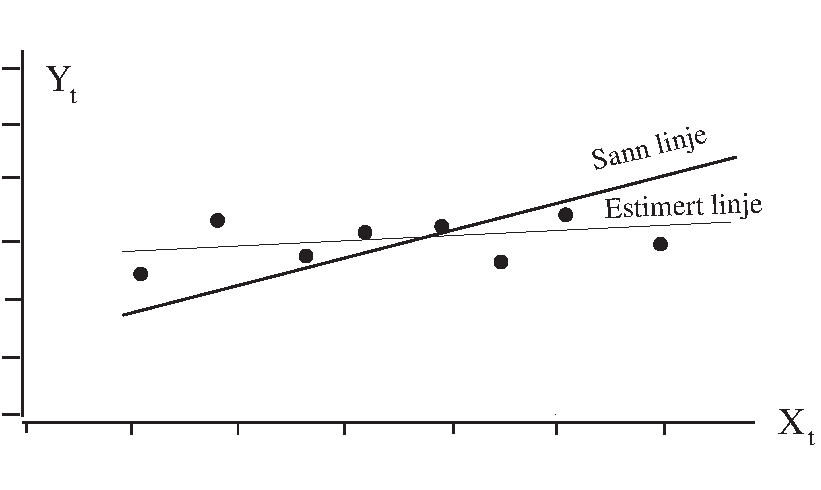
\includegraphics[scale=0.7]{figurer/fig13_10.pdf} 
 \caption{Regresjon og positiv autokorrelasjon}
	\label{fig:regresjon_acf}
\end{figure}

I Figur~\ref{fig:regresjon_acf} har vi tegnet inn den sanne regresjonslinjen med hel strek, samt en
tidsrekke som svarer til at feilleddene har positiv autokorrelasjon
\footnote{Her var forklaringsvariablen tiden selv, men situasjonen er i
prinsippet den samme for alle forklaringsvariable med verdier som
gjennomgående er korrelert med $t$.},
dvs. positive (negative) avvik fra regresjonslinje etterfølges 
gjennomgående av positive (negative) avvik.  Vi har gått ut fra at det
første avviket fra regresjonslinjen tilfeldigvis var positivt, og 
tidsrekken vil da typisk kunne ha et forløp som vist på figuren.  Vi 
ser at analyse basert på den observerte rekken uten kunnskap om
autokorrelasjon, vil gi en estimert linje som stiplet på figuren.
Vi ser at vi har underestimert regresjonskoeffisienten $\beta$.  Tilsvarende
dersom vi tilfeldigvis startet med et negativt feilledd ville vi antakelig
overestimere regresjonskoeffisienten.  Det som er spesielt infamt er at vi
tilsynelatende har fått god tilpasning til en rett linje, men linjen
ligger altså ikke på rett sted.  Et forsøk på å estimere
variansen til feilleddet på grunnlag av residualene vil, med den rekken
som er illustrert i figuren, totalt undervurdere denne.  Vi vet heller ikke om
vi har eventuelt over- eller underestimert regresjonskoeffisienten.  Dersom
vi hadde fortsatt å observere tidsrekken en tid ville den høyst
sannsynlig krysse den sanne linjen igjen, slik at sjansen for å gå
i fellen er redusert.

De forhold som her er belyst har en viss betydning for den analyse av trend
og sesongvariasjon som ble foretatt i avsnitt 13.2 basert på
regresjons\-modellen, og kan også forkludre andre analysemetoder.
Dersom det også er autokorrelasjon til stede, vil denne kunne feilaktig
bli tolket som trend eller sesongvariasjon, selv om vi har 
fått god lineær tilpasning til modellen.

Det finnes ulike måter å unngå slike feller som er beskrevet
ovenfor, men disse vil avhenge noe av hvilke typer tidsavhengighet man
ønsker å gardere seg mot.  Vi vil her kort se på situasjonen
dersom man er villig til å representere feilleddet med en første
ordens autoregressiv modell, dvs.

\[ U_t= \rho U_{t-1} + V_t \; \; \; t=1,2, \ldots , n     \]

\noindent der $V_t$'ene er uavhengige avvik med forventning null og samme
varians. Med utgangspunkt de observerte rekkene $Y_1, Y_2, \ldots, Y_n$ og
$X_1, X_2,\ldots, X_n$ beregner vi

\[ Y_t^{'}=Y_t-\rho Y_{t-1}  \mbox{\ \ \ }  X_t^{'}=X_t-\rho X_{t-1}  \]

\noindent Vi ser at ifølge regresjonsmodellen
$Y_t = \gamma + \beta X_t + U_t$, kan vi skrive
 \footnote{Vi ser at $Y_t^{'}$ og $X_t^{'}$ ikke lar seg beregne for
$t = 1$. Det er da vanlig å isteden sette $Y_1^{'} =\sqrt{1-{\rho}^2}Y_1$
og $X_1^{'} =\sqrt{1-{\rho}^2}X_1$ , hvorfor kan vi ikke gå inn på her.}  

\[Y_t^{'} = \gamma(1-\rho) + \beta X_t^{'} + V_t \]

\noindent slik at vi har en regresjon som oppfyller antakelsene i 
standardregresjonsmodellen, der $\beta$ kan estimeres på vanlig måte
uten problemer.

Den metode som er foreslått ovenfor lar seg gjennomføre dersom vi
kjenner $\rho$, men dette er som regel ikke tilfelle.  Vi merker oss at
regre\-sjons\-koef\-fisienten i den avledede modell er $\beta$ uansett
hvilken $\rho$ som brukes.  Det er derfor aktuelt å bruke $\rho = 1$, dvs.
sette $Y_t^{'} = Y_t - Y_{t-1}$ og $X_t^{'} = X_t - X_{t-1}$. Det viser seg at
faren for feilestimering av $\beta$ nå er betydelig redusert, uansett hva
$\rho$ virkelig er.  Et alternativ til dette vil være å estimere $\rho$
på grunnlag av (en del av) den observerte rekke.  Ut fra den 
autoregressive modellen for feilleddet $U_t$, ser det ut til at vi kan 
estimere $\rho$ på samme måte som tilfellet var i avsnitt 13.3.  Dette
forutsetter imidlertid at feilleddene $U_t$ lar seg observere, men det kan
de jo ikke.  Det beste vi kan gjøre synes å være å estimere
regresjonslinjen ${\hat{Y}}_t = \hat{\gamma} + {\hat{\beta}}\cdot X_t$ på
vanlig måte med minste kvadraters metode, og deretter beregne residualene
${\hat{U}}_t = Y_t - {\hat{Y}}_t$ og bruke disse istedenfor $U_t$ ved estimering av
$\rho$.  Dette gir estimatoren

\[ \hat{\rho}=\frac{\sum_{t=2}^n {\hat{U}}_{t-1}{\hat{U}}_t}
                   {\sum_{t=1}^n {\hat{U}}_t^2}  \]
\noindent Av Figur~\ref{fig:regresjon_acf} ser vi imidlertid at denne antakelig vil underestimere
$\rho$ idet variasjonen omkring den estimerte linje ser mer tilfeldig ut enn
omkring den sanne linjen.  Det finnes metoder som korrigerer denne
underestimeringen.

Vi vil ofte ved gjennomføringen av en regresjonsanalyse etter vanlige 
metoder være interessert i å teste om feilleddene med rimelighet kan
antas uavhengige, slik at forutsetningene i standardregresjonsmodellen er
oppfylt.  Vår mulighet ligger i å se på residualene $\hat{U_t}$
etter regresjonsanalysen.  Den testen som vanligvis utføres er
{\em Durbin-Watsons test} som forestiller seg at alternativet til hypotesen
om uavhengighet er første ordens autoregresjon.  Problemstillingen kan
derfor oppfattes som å teste $\rho =0 $ mot alternativet $\rho > 0 $ (evt.
$\rho < 0 $).  Durbin-Watson testobservatoren er (jfr. Oppgave~17)

\[ D=\frac{\sum_{t=2}^n {({\hat{U}}_t-{\hat{U}}_{t-1})}^2} 
          {\sum_{t=1}^n {{\hat{U}}_t}^2}  \approx 2(1-\hat{\rho}) . \]

\noindent Liten verdi av $D$ gir grunn til å påstå positiv
autokorrelasjon.
Tabell~\ref{tab:Durbin_Watson_test} i Appendiks~\ref{app:fordelngstabeller} gir kritiske verdier for $D$ svarende til 5\% signifikansnivå.
En $D$ lavere enn tabellverdien $d_L$ betyr klar forkastning av hypotesen om
uavhengighet til fordel for positiv autokorrelasjon.
En verdi mellom $d_L$ og $d_U$ gir svak indikasjon på positiv 
autokorrelasjon, mens en verdi mellom $d_U$ og 2 gir klar indikasjon på at
hypotesen om uavhengighet er rimelig. Med negativ auto\-korrelasjon som (ensidig)
alternativ brukes samme rettesnor, men med $D^{'}=4-D$ som testobservator
istedenfor D.


De forhold som er diskutert ovenfor gjelder også for regresjons\-ana\-lyse
med mer enn en forklaringsvariabel, og testobservatoren for testing av
uavhengige feilledd har samme form. Sannsynlighetsfordelingen til $D$ vil
avhenge av antall forklarende variable $r$, og i Tabell~\ref{tab:Durbin_Watson_test} er 
de kritiske verdier gitt i separate kolonner for ulike $r$.
Durbin-Watson testen med rapport av P-verdier fins som regel som opsjon i 
programvare.
 

I praksis er det nok bare i tilfellet med klar forkasting av hypotesen om
uavhengighet at en standard regresjonsanalyse diskrediteres, og en ser seg om
etter en alternativ metode som fanger opp autokorrelasjonen, f.eks.
som antydet ovenfor. I situasjonen med svak autokorrelasjon har man ingen
garanti for at en alternativ metode gir et mer pålitelig resultat, men det
er et spørsmål om sunt omdømme. \\

\begin{eksempel}{Omsetning}
Vi studerer igjen tidsrekken bestående av kvartalsvise omsetningstall
som er gitt i Eksempel 3, og analysert i Eksempel 4 på grunnlag av en
regre\-sjons\-modell med fire forklaringsvariable.  Beregning av residualene
ga som resultat (sjekk og tegn figur!) 
\begin{center}
\begin{tabular}{rrrrrrr}
     0.62  &  0.42  &  $-0.31$  &  $-0.97$  &  0.00  &  1.00  &  $-0.53$ \\
     0.00  & $-0.63$  &  $-1.42$  &   0.84  &  0.97  &        &
\end{tabular}
\end{center}
Det gir $D = 1.69$ som ifølge Tabell~\ref{tab:Durbin_Watson_test} ikke er tilstrekkelig lite til
å påstå positiv autokorrelasjon.  Vi føler oss derfor 
noenlunde trygge på den analysen som ble foretatt i Eksempel 4, og 
korreksjon for autokorrelasjon synes derfor ikke aktuelt.
\end{eksempel}

La oss ta for oss et avsluttende mer realistisk eksempel.\\

\begin{eksempel}{Salg-Reklame}
La oss igjen ta for oss dataene fra Eksempel 1.9, der vi observerte
sammenhørende verdier av reklameinnsats $X$ (i tusen kroner) og solgt
kvantum $Y$ i etterfølgende perioder. Anta at det er kvartalsvise data
over tre år :
 \begin{center} \small \addtolength{\tabcolsep}{-0.4\tabcolsep}
  \begin{tabular}{lcccccccccccc}
  Periode:  & 1&2&3&4&5&6&7&8&9&10&11&12 \\
  Kvartal: & 1&2&3&4&1&2&3&4&1&2&3&4 \\
       X: & 4.0&2.0&2.5&2.0&3.0&5.0&4.0&2.0&5.0&4.0&2.5&5.0 \\
       Y: &385&400&395&365&475&440&490&420&560&525&480&510 \\
  \end{tabular}
 \end{center}
La oss tenke oss muligheten av at det i tillegg til reklameeffekten er både
lineær trend og sesongvariasjon. En slik analyse, som samtidig kan 
indikere om det skulle være autokorrelasjon, er gitt i utskrift nedenfor.

Med reklame som eneste forklaringsvariabel var denne klart signifikant.
Durbin-Watson observatoren er $D$=1.35, som indikerer en
svak positiv autokorrelasjon (ikke signifikant).
Vi ser til vår forundring at tidstrend har slått ut reklamen
som for\-kla\-rende variabel i den utvidede modellen. Videre ser vi at
4. kvartal er lavsesong i forhold til 1. kvartal, mens 2. og 3. kvartal er
mellomsesong, som riktignok ikke er signifikant forskjellig fra 1. kvartal.
Forklaringsgraden er også økt fra 40.3\% til hele 90.5\%, mens
standardavviket til feilleddet er redusert fra $S$=50.23 til $S$=25.86.
Dette indikerer at den siste modellen kan ha betydelig bedre prediksjonsevne.
Endelig ser vi at Durbin-Watson observatoren er $D$=2.65, som indikerer en
svak negativ autokorrelasjon (ikke signifikant).

\begin{center} \framebox[11cm]{\begin{minipage}{10cm}\rule{0cm}{0.5cm}
\tt
 >> READ 'eks1.9' X Y \\
\ \ >> SET T = 1:12\\
\ \ >> SET S = 3(1:4)\\
\ \ >> INDICATOR S in S1 S2 S3 S4\\
\ \ >> REGRESS Y on X ; DW.\\
   Y = 344 + 32.2 X  (S=50.23)\\
\begin{tabular}{rrrrr}
            &           &  St.Dev   & T-ratio  &       \\
  Variable  &Coefficient&  of Coef. & Coef/S.D.&       P\\
            &   343.71  &    44.77  &    7.68  &   0.000\\
  X         &    32.21  &    12.40  &    2.60  &   0.027
\end{tabular}\\
  Degrees of freedom for T-test  = 10 \\
  R-squared = 40.3\%   (Adjusted for d.f. = 34.3\%)\\
  Durbin-Watson statistic = 1.35 \\[1mm]
\ \ >> REGRESS Y on X T S2 S3 S4 ; DW.\\
  Y = 368 + 7.24 X + 15.2 T\\
 \mbox{\ \ \ \ \ \ }         - 31.1 S2 - 41.5 S3 - 80.0 S4  (S=25.86)\\
\begin{tabular}{rrrrr}
             &           &  St.Dev   & T-ratio  &       \\
  Variable   &Coefficient&  of Coef. & Coef/S.D.&       P\\
             &  368.34  &     31.67  &    11.63 &   0.000 \\
  X          &   7.241  &     8.319  &     0.87 &   0.418 \\
  T          &  15.205  &     2.768  &     5.49 &   0.002 \\
  S2         &  -31.12  &     21.68  &    -1.44 &   0.201 \\
  S3         &  -41.50  &     24.45  &    -1.70 &   0.141 \\
  S4         &  -80.04  &     25.73  &    -3.11 &   0.021
\end{tabular}\\
  Degrees of freedom for T-test  = 6 \\
  R-squared = 90.5\%   (Adjusted for d.f. = 82.6\%)\\
  Durbin-Watson statistic = 2.65
\mbox{}\\
\end{minipage}} \end{center}



Vi bør imidlertid summe oss litt her : Studerer vi tallene litt nærmere,
ser vi at det er en tendens til at reklameinnsatsen er økt over  tid.
Det er derfor vanskelig å avgjøre om økt salg skyldes reklameinnsats,
tidstrend eller begge deler. Videre ser vi at reklameinnsatsen gjennomsnittlig
var større i 1. kvartal enn de øvrige, og det er derfor vanskelig å
 si om det virkelig er en sesongeffekt eller om den delvis skyldes mer reklame.
\end{eksempel}

Dette eksemplet viser igjen hvor vanskelig det er å trekke generelle 
konklusjoner i situasjoner der data ikke er planmessig innsamlet. Hvis vi
virkelig ønsket å undersøke reklameeffekten alene, må vi
søke å variere reklamen over tiden og for de ulike kvartaler i 
henhold til en plan som unngår at de forklarende variable blir korrelerte.\\
 

\normalsize


\section{Oppgaver}
\small
\begin{enumerate}
\item Dekomponer tidsrekken i Eksempel 3 etter modellen $Y_t = T_t + S_t +
U_t$ og gi prognoser for kommende år.  Drøft valget av 
dekomponeringsmetode for denne rekken.

\item Gitt følgende tidsrekke med kvartalsvise økonomiske data over
en periode på fire år 
\begin{center}
\begin{tabular}{lcccccccc}
 $Y_t$: &  14.0  &  16.2  &  18.3  &  20.5  &  15.6  &  22.1  &  18.4 & 27.2 \\
     &  18.9  &  22.0  &  24.8  &  26.8  &  16.9  &  24.0  &  26.9  &  27.7
\end{tabular} 
\end{center}
\begin{itemize}
\item[(a)] Tegn denne tidsrekken i en figur, og tegn inn eventuell trend.
\item[(b)] Dekomponer tidsrekken etter modellen $Y_1 = T_tS_tU_t$, der
           sesongperioden er et år.
\item[(c)] Gi en prognose for tidsrekkens verdier neste år.
\end{itemize}
\item  Anta at tidsrekken i Oppgave~2 er en fortsettelse av tidsrekken i
 Eksempel 3, slik at vi har observert rekken i alt over en periode på syv
 år. Vi vet at i skillet mellom de to observasjonsperiodene fant det sted
 en endring i de økonomiske forhold.  
\begin{itemize}
\item[(a)] Tyder observasjonene på at trenden er forskjellig i de to 
         periodene ?  Hvis ikke anslå en felles trend for hele materialet.
\item[(b)] Tyder observasjonene på at sesongfaktoren kan være lik for
   de to periodene.  Fastlegg i så fall sesongfaktorene på grunnlag av
    hele materialet og gi nye prognoser for neste år.
\end{itemize}
\item Gitt følgende tidsrekke som er en alternativ fortsettelse av
      tidsrekken i Eksempel 3 : 
\begin{center}
\begin{tabular}{lccccccccc}
 $Y_t$: &  12.3  &  13.5  &  16.0  &  20.4  &  15.8  &  17.1  &  18.0  & 27.7\\
     &  20.8  &  24.3  &  26.4  &  30.0  &  24.0  &  30.8  &  24.3  &  34.8
\end{tabular}
\end{center}
Drøft om tidsrekken kan ha endret karakter ved tidsskillet.

\item Enkelte tidsrekker kan ved tidsskiller få et skift, dvs. at rekken
 med utgangspunkt i et nytt nivå i hovedsak utvikler seg som før.
\begin{itemize}
\item[(a)] Forklar at dette kan analyseres innenfor en lineær modell,
           f.eks. slik
      \[Y_t={\beta}_0+{\beta}_1 t+{\beta}_2 Q+{\beta}_3 I+U \]

\noindent der $I$ er en indikatorvariabel med verdi 0 før tidsskillet
         og 1 etter.
\item[(b)] Tolk parametrene i modellen i (a).
\item[(c)] $\star$Utfør en analyse basert på en modell av denne typen
       (med tre sesongvariable) og med hele tallmaterialet fra Eksempel 3 og
      Oppgave~4.
\end{itemize}

\item Drøft hvilke problemer som oppstår ved analyse av tidsrekker der
    vi på forhånd ikke vet om eventuelle tidsskiller der rekken kan ha 
    endret karakter.

\item Det foreligger en tidsrekke $Y_t$ av kvartalsvise data med trend og
    sesongvariasjoner der vi vet at sesongkomponenten har en syklisk karakter,
    dvs. jevnt stigende fra lavsesong til høysesong og ned igjen over en
    periode på et år.
\begin{itemize}
\item[(a)] Drøft bruk av følgende modell

      \[Y_t={\beta}_0+{\beta}_1 t+{\beta}_2 sin(2\pi k/4)+U_t \]

\noindent der $k$ betegner kvartal nr.$k = 1, 2, 3, 4.$
\item[(b)] Lag tilsvarende modell dersom tidsrekken er observert 
           månedsvis.
\item[(c)] Hvilken teknikk er aktuell for analyse av slike modeller?
\end{itemize}

\item Gitt følgende tidsrekke som antas å være uten trend og 
      sesongvariasjoner :
\begin{center} \addtolength{\tabcolsep}{-0.2\tabcolsep}
\begin{tabular}{lrrrrrrrrrr}
$Y_t$:& 0.9 & 2.2 & 1.2 &$-0.9$&$-0.3$&$-1.7$& 0.6 & 1.7 &$-0.8$&$-2.3$ \\
      &$-1.5$&$-0.7$&2.1&0.6&$-0.8$&$-1.9$&$-1.2$& 0.8 & 1.4 & 1.0 \\
\end{tabular}
\end{center}
\begin{itemize}
\item[(a)] Viser denne rekken tegn til autokorrelasjon?
\item[(b)] Estimer en første orden autoregressiv modell.
\item[(c)] Prediker de to neste verdiene av rekken.
\end{itemize}

\item Betrakt AR(1) modellen 
       \[ Y_t= \gamma +\rho Y_{t-1} + U_t \]
      der $U_t$'ene er uavhengige med samme varians ${\tau}^2$.
      Vis at (ubetinget) forventning og varians er gitt ved
      \[ \mbox{\ \ (i)\ \ } \mu = \gamma /(1-\rho ) \mbox{\ \ \ \ (ii)\ \ }
                                    {\sigma}^2 = {\tau}^2/(1-{\rho}^2) \]
      Kan du også si noe om betingede forventninger og varianser?
\item Betrakt en {\em ``random walk''}
       \[ Y_t=Y_{t-1}+U_t \]
      der $U_t$'ene er uavhengige med samme varians ${\tau}^2$.
      Undersøk egenskapene: forventning, varians etc.

\item Vis at en AR(1) tidsrekke har autokovariansfunksjon med form
\[   c(k)={\rho}^kc(0) \mbox{\ \ \ } k=0,1,2,\ldots         \]
Kommenter resultatet.

\item Vis at en MA(1) tidsrekke har autokovariansfunksjon med form
\[ c(0)=(1+{\alpha}^2)\cdot {\tau}^2,  \; \;c(1)={\alpha} \cdot {\tau}^2, \; \;
                         c(k)=0 \mbox{\ \ \ for \ \ } k \ge 2. \]
Kommenter resultatet.
\item Anta  en første ordens autoregressiv tidsrekke
  $Y_t = \rho Y_{t-1} + U_t$ der $\rho$ er kjent, og $U_t$'ene uavhengige
 variable med forventning null og varians ${\sigma}^2$.

\begin{itemize}
\item[(a)] Rettferdiggjør bruk av ${\hat{Y}}_{n+k} = {\rho}^kY_n$ som
 prediktor $k$ skritt fram i tid fra tidspunkt $n$.
\item[(b)] Vis at prediksjonsfeilen
 ${\hat{U}}_{n+k} = Y_{n+k} - {\hat{Y}}_{n+k}$
har forventning null og varians
\[ (1+{\rho}^2+{\rho}^4+ \cdots +{\rho}^{2(k-1)}){\sigma}^2 \]
Kommenter resultatet.
\end{itemize}

\item Som prognose for verdien av en tidsrekke ett skritt fram i tid,
  er valgt den sist observerte verdi dvs.
\[ {\hat{Y}}_{t+1}=Y_t \mbox{\ \ \ } t=1,2,3,\ldots    \]
Finn forventningen og variansen til prediksjonsfeilen ${\hat{U}}_{t+1} =
Y_{t+1} - {\hat{Y}}_{t+1}$ dersom
\begin{itemize}
\item[(a)] $Y_t = {\gamma} + {\beta}t + U_t$    \mbox{ (lineær trend)}
\item[(b)] $Y_t = \gamma + \rho Y_{t-1}+U_t$    \mbox{(autoregresjon)}
\item[(c)] $Y_t = \mu +\alpha U_{t-1}+U_t$       \mbox{(glidende gjennomsnitt)}
\end{itemize}
\noindent der $U_t$'ene er uavhengige variable med forventning null og
 varians ${\tau}^2$.

\item En prognosemetode kalt {\em eksponensiell glatting} er gitt ved
 formelen
\[ {\hat{Y}}_{t+1}= aY_t+(1-a){\hat{Y}}_t \] 
\noindent dvs. prognosen på tidspunkt $t$ for neste verdi av tidsrekken er
 en veid sum av observert verdi av rekken på tidspunkt $t$ og prognosen
 for dette tidspunkt foretatt på $t - 1$.  Dersom vi starter med prognoser
 på tidspunkt $n$ trengs en startverdi $\hat{Y}_n$ som velges etter beste 
 skjønn.  

\begin{itemize}
\item[(a)] Drøft valg av a.
\item[(b)] Fyll inn prognoser og sammenlign med de virkelig observerte
verdier dersom vi velger (i) $a = 0.2$  (ii) $a = 0.5$ \\
\begin{tabular}{rcccccc}
 $t$:         & n   &   n+1   &   n+2   &   n+3   &   n+4   &   n+5 \\
 $\hat{Y_t}$:&0.0&($\ldots $)&($\ldots $)&($\ldots $)&($\ldots $)&($\ldots $)\\
 $Y_t$:       & 1.0 &   1.0   &   0.0   &   1.0   &   2.0   &   2.0
\end{tabular}
\item[(c)] Vis at denne prognosemetoden ikke er brukbar dersom tidsrekken
har negativ autokorrelasjon.
\item[(d)] Vis at denne prognosemetoden ikke gir gode resultater for 
tidsrekker med trend (jfr. Oppgave~14).
\end{itemize}

\item Følgende modell for autokorrelasjon er foreslått

\[   Y_t=\beta Y_{t-1}+\beta (1-\beta)Y_{t-2}+\beta {(1-\beta)}^2 Y_{t-3}
                         + \cdots + U_t \]
\noindent der $\beta$ er tall mellom 0 og 2 som uttrykker graden av
          autokorrelasjon.
\begin{itemize}
\item[(a)] Tolk denne modellen.
\item[(b)] Under hvilke forutsetninger er det rimelig å bruke 
prediktoren
\[  {\hat{Y}}_t=\beta Y_{t-1}+\beta (1-\beta)Y_{t-2}
                    +\beta {(1-\beta)}^2 Y_{t-3}+ \cdots   \]
\item[(c)] Vis at
\[   {\hat{Y}}_{t+1} = \beta Y_t + (1 - \beta){\hat{Y}}_t \]
\noindent og kommenter resultatet i lys av prognosemetoden i forrige oppgave.
\end{itemize}

\item $Y_1, Y_2, \ldots, Y_n$ er uavhengige med forventning $\mu$
og varians $\sigma^2$. Betrakt
\[ D=\frac{C^2}{S^2}=\frac{ \frac{1}{n-1}\sum_{t=2}^n {(Y_t-Y_{t-1})}^2}
                       { \frac{1}{n-1}\sum_{t=1}^n {(Y_t-\bar{Y})}^2}  \]
Vis at $EC^2 =2 {\sigma}^2$ og forklar at $D$ antar verdier mellom 0 og 4.
Forklar videre at $D\approx 2$ indikerer uavhengighet, mens verdier som er noe
mindre/større enn 2 indikerer hhv. positiv  og negativ autokorrelasjon
(av første orden). 

\item
Gitt følgende tidsrekke: 
\begin{center}
\begin{tabular}{rrrrrrrrrrr}
$Y_t$: & 5.9  &  7.3 &  8.5 &  9.2 &  9.9 & 10.6 & 11.8 & 12.3 & 13.7 & 15.2 \\
     &16.7  & 17.4 & 18.7 & 19.2 & 20.1 & 21.2 & 21.8 & 22.5 & 23.7 & 24.4
\end{tabular}
\end{center}
Som modell er valgt $Y_t = \gamma +{\beta}t + U_t$, dvs. lineær trend 
uten sesongvariasjoner.

\begin{itemize}
\item[(a)] Tegn tidsrekken i en figur og drøft om modellen synes rimelig.
\item[(b)] Estimer minste kvadraters regresjonslinje.
\item[(c)] Beregn residualene og drøft om feilleddene $U_t$ kan være
autokorrelerte.
\item[(d)] Utfør Durbin-Watsons test for uavhengighet.
\end{itemize}

\item Utfør flere regresjonsanalyser på dataene i Eksempel 10.
     \begin{itemize}
     \item[(a)] med reklame og tid som forklarende variable, 
              uten å ta omsyn til sesongvariable,
     \item[(b)] med reklame i forrige periode som ekstra forklaringsvariabel.
     \end{itemize}
      Kommenter resultatene. 

\item For å bli kjent med karakteren av ulike typer tidsrekker,
kan disse simuleres med programvare på en PC.  Samtidig kan en studere de 
relative fortrinn av ulike prognosemetoder under ulike omstendigheter.
Studer mulighetene for å foreta slike analyser med den programvare
du har til rådighet.

\item Undersøk tilgjengelig statistisk programvare kan tilby analyse og
      prediksjon av tidsrekker . Finn ut hvilke typer modeller
      som ligger til grunn.
      Undersøk også om hvilke elementer, trend, sesongvariasjon, 
      autokorrelasjon osv. som programvaren fanger opp.
 
\end{enumerate}
\normalsize
